\documentclass[aspectratio=169,13pt,fleqn,t] {beamer}
%
% Choose how your presentation looks.
%
% For more themes, color themes and font themes, see:
% http://deic.uab.es/~iblanes/beamer_gallery/index_by_theme.html
%
\mode<presentation>
{
	\usetheme{Madrid}      % 整体主题
	\usecolortheme{beaver} % 配色主题（棕红系）
	\usefonttheme{serif}   % 全局衬线字体（正文宋体类）
	\setbeamertemplate{items}[default] % 【items父模板】控制 itemize+enumerate 符号
%	\setbeamertemplate{items}{\Large\beamertemplateballitem}
	\setbeamertemplate{sections/subsections in toc}[ball] % 目录里章节用圆圈标记
	
	%  \setbeamertemplate{navigation symbols}{} % 取消注释可隐藏底部导航小图标
	\setbeamertemplate{caption}[numbered] % 图/表标题带编号：图1、表1
}

\usepackage[,UTF8,linespread=1.2]{ctex}
\usepackage{wrapfig}
\usepackage{caption}
\usepackage{tcolorbox}
\tcbuselibrary{skins}
\captionsetup[figure]{name=图,labelsep=period}
\usepackage{pdfpages}
\usepackage{tabularx,array}
\usetikzlibrary{arrows.meta,intersections,positioning}

\usepackage{xcolor}
\definecolor{xy_blue}{cmyk}{0.6,0.35,0.0,0.4}
\definecolor{xy_orange}{cmyk}{0.0,0.7,1.0,0.0}
\definecolor{xy_green}{cmyk}{0.2,0.0,1.0,0.15}
\xdefinecolor{xy_gold}{RGB}{135,103,79}
\xdefinecolor{xy2_gold}{cmyk}{0,0.35,0.75,0.05}

\setbeamercolor{section number projected}{fg=red,bg=red!20}%控制球的颜色
\setbeamercolor{subsection number projected}{fg=blue,bg=blue!40}
\setbeamercolor{item}{fg=xy_gold} %设置列表项颜色

\usepackage{amsthm}
\newtheorem{peroration}{结论：}
\newtheorem*{exploration}{探究：}
\newtheorem*{prooft}{证明：}
\newtheorem*{solve}{解:} 
\newtheorem{instance}{例}   % 解：独立计数器
\newtheorem*{definate}{定义：}
     

% 配色（你前面需要的，每个环境单独颜色）
\setbeamercolor{theorem}{fg=black,bg=blue!10}
\setbeamercolor{solution}{fg=black,bg=green!10}

\BeforeBeginEnvironment{peroration}{%结论： 
	\setbeamercolor{block title}{bg=xy_green,fg=white}
	\setbeamercolor{block body}{bg=xy_green!10}
}
\AfterEndEnvironment{peroration}{
	\setbeamercolor{block title}{bg=xy_blue,fg=white}
	\setbeamercolor{block body}{bg=xy_blue!10}
}
\BeforeBeginEnvironment{exploration}{%探究
	\setbeamercolor{block title}{bg=xy_orange,fg=white}
	\setbeamercolor{block body}{bg=xy_orange!10}
}
\AfterEndEnvironment{peroration}{
	\setbeamercolor{block title}{bg=xy_blue,fg=white}
	\setbeamercolor{block body}{bg=xy_blue!10}
}
\BeforeBeginEnvironment{solution}{%解
	\begingroup
	\setbeamercolor{block title}{bg=xy_green,fg=white}
	\setbeamercolor{block body}{bg=xy_green!10}
}
\AfterEndEnvironment{solution}{
	\endgroup
}
\BeforeBeginEnvironment{prooft}{%证明
	\setbeamercolor{block title}{bg=xy_green,fg=white}
	\setbeamercolor{block body}{bg=xy_green!10}
}
\AfterEndEnvironment{prooft}{
	\setbeamercolor{block title}{bg=xy_green,fg=white}
	\setbeamercolor{block body}{bg=xy_green!10}
}
\BeforeBeginEnvironment{solve}{%解：
	\setbeamercolor{block title}{bg=xy_orange!60,fg=white}
	\setbeamercolor{block body}{bg=xy_orange!10}
}
\AfterEndEnvironment{solve}{%解：
	\setbeamercolor{block title}{bg=xy_orange!60,fg=white}
	\setbeamercolor{block body}{bg=xy_orange!10}
}
   
\BeforeBeginEnvironment{instance}{% 例子
	\begingroup
   	\setbeamercolor{block title}{bg=xy_gold!40,fg=white}
   	\setbeamercolor{block body}{bg=xy_gold!10}
   }
\AfterEndEnvironment{instance}{
	\endgroup
   }     
   
\renewcommand{\thefigure}{\arabic{figure}}

\title[2.3~一元二次不等式]{2.3~~二次函数与一元二次方程、不等式(应用)}
\author[好好学习，努力向上]{}
\institute{}
\date{2026.9.29}
\setbeamertemplate{theorems}[numbered]

\AtBeginSection[]
{
  \begin{frame}<beamer>
    \frametitle{本节主要内容}
    \tableofcontents[currentsection,currentsubsection]
  \end{frame}
}

\AtBeginDocument{
	\setlength{\abovedisplayskip}{3pt}
	\setlength{\belowdisplayskip}{3pt}
	}


\begin{document}
\begin{frame}{}
	\titlepage
\end{frame}

\begin{frame}{内容概览}
	\tableofcontents
\end{frame}

\section{前情回顾}

	
	
	\begin{frame}[t]{前情回顾---一元二次不等式与二次函数、一元二次方程的关系}
		\small
		\begin{tabularx}{\textwidth}[c]{|*{4}{>{\arraybackslash}m{3.37cm}|}}
			\hline
			\centering 项目 &	\centering $\Delta>0$	& \centering$\Delta=0$	&	\centering\arraybackslash$\Delta<0$	\\
			\hline
			$y=ax^2+bx+c(a>0)$的图象	&	
			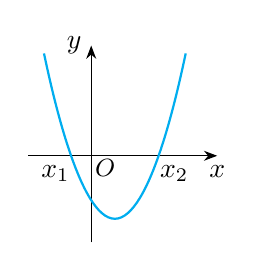
\begin{tikzpicture}[baseline={(0,-1)}]
				\draw[-Stealth,name path=line](-0.8,0) -- (1.6,0)node[below]{$x$};
				\draw[-Stealth](0,-1.1) -- (0,1.4)node[left]{$y$};
				\draw[thick,cyan,name path=curve](-0.6,1.3) parabola bend(0.3,-0.8) (1.2,1.3);
				\path[name intersections={of= line and curve,name=t}]
				(t-1)node[below left= 0pt and  -3pt]{$x_1$}
				(t-2)node[below right= 0pt and  -3pt]{$x_2$};
				\node[below right=-3pt] at (0,0){\small $O$};
			\end{tikzpicture}	&	
			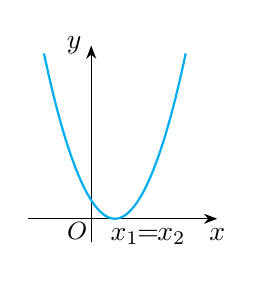
\begin{tikzpicture}[baseline={(0,-1)}]
				\draw[-Stealth,name path=line](-0.8,-0.8) -- (1.6,-0.8)node[below]{$x$};
				\draw[-Stealth](0,-1.1) -- (0,1.4)node[left]{$y$};
				\draw[thick,cyan,name path=curve](-0.6,1.3) parabola bend(0.3,-0.8) (1.2,1.3);
				\path[name intersections={of= line and curve,name=t}]
				(t-1)node[below right =0pt and -5pt ]{$x_1\!\!=\!\! x_2$};
				\node[below left=-3pt] at(0,-0.8){\small $O$};			
			\end{tikzpicture}		&	
			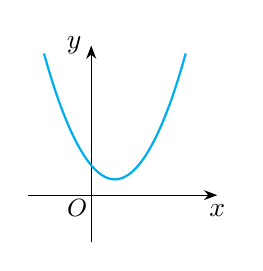
\begin{tikzpicture}[baseline={(0,-1)}]
				\draw[-Stealth,name path=line](-0.8,-0.5) -- (1.6,-0.5)node[below]{$x$};
				\draw[-Stealth](0,-1.1) -- (0,1.4)node[left]{$y$};
				\draw[thick,cyan,name path=curve](-0.6,1.3) parabola bend(0.3,-0.3) (1.2,1.3);			
				\node[below left=-3pt] at(0,-0.5){\small $O$};			
			\end{tikzpicture}	\\
			\hline
			$ax^2+bx+c=0(a>0)$的根	&	有两个不相等的实数根$x_1,x_2(x_1<x_2)$	&	有两个相等的实数根$x_1=x_2=-\frac{b}{2a}$	&	没有实数根	\\
			\hline
			$ax^2+bx+c>0(a\neq 0)$的根	&$\{x\mid x<x_1,\text{或} x>x_2\}$	&	$\{x\mid x \neq -\frac{b}{2a}\}$	&	\centering\arraybackslash$\mathbf{R}$		\\
			\hline
			$ax^2+bx+c<0(a>0)$的解集	&	\centering$\{x \mid x_1<x<x_2\}$		&	\centering$\varnothing$	&	\centering\arraybackslash$\varnothing$	\\
			\hline
		\end{tabularx}
		%\vspace{-2em}
		%\begin{figure}
		%	\includegraphics[height=7.5cm]{Figures/budengshi.png}
		%\end{figure}
		
	\end{frame}
	


\section{一元二次不等式的应用}
\begin{frame}[t]{一元二次不等式的应用(一)}
\begin{instance}
	一家车辆制造厂引进了一条摩托车整车装配流水线，这条流水线生产的摩托车数量 \(x\)（单位：辆）与创造的价值 \(y\)（单位：元）之间有如下关系：
	\[
	y = -20x^2 + 2200x.
	\]
	若这家工厂希望在一个星期内利用这条流水线创收 $60\,000$ 元以上，则在一个星期内大约应该生产多少辆摩托车？
\end{instance}
\end{frame}

\begin{frame}[t]

	\begin{solve}
		\begin{wrapfigure}[14]{r}{5cm}
			\begin{center}			
			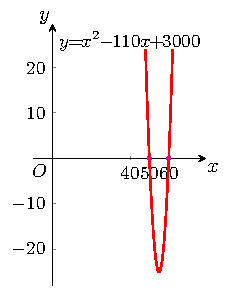
\includegraphics{Figures/budengshi1.pdf}
			\caption{}\label{fig:fig1}
			\end{center}
		\end{wrapfigure}
		设这家工厂在一个星期内大约应该利用这条流水线生产\(x\)辆摩托车，根据题意，得		
		\[
		-20x^2 + 2200x > 60\,000.
		\]		
		移项整理，得$x^2 - 110x + 3000 < 0.$
		
		解方程\quad \(x^2 - 110x + 3000 = 0\)，得 \(x_1 = 50\)，\(x_2 = 60\).
		
		 画出二次函数 \(y = x^2 - 110x + 3000\) 的图象\textup{(如图\ref{fig:fig1})}，
		 
		 结合图象得不等式 \quad \(x^2 - 110x + 3000 < 0\) 的解集为 \(\{x \mid 50 < x < 60\}\)，从而原不等式的解集为
		 \[
		\{x \mid 50 < x < 60\}.
		\]
		因为 \(x\) 只能取整数值，所以当这条流水线在一周内生产的摩托车数量在 \(51 \sim 59\) 辆时，这家工厂能够获得 $60\,000$ 元以上的收益.
	\end{solve}
\end{frame}

\begin{frame}[t]{一元二次不等式的应用(二)}

	\begin{instance}
		某种汽车在水泥路面上的刹车距离 \(s\)（单位：m）和汽车刹车前的车速 \(v\)（单位：km/h）之间有如下关系：
		\[
		s = \frac{1}{20}v + \frac{1}{180}v^2.
		\]
		在一次交通事故中，测得这种车的刹车距离大于 $39.5\; m$，那么这辆汽车刹车前的车速至少为多少（精确到 $1\; km/h$）？
	\end{instance}
\end{frame}



\begin{frame}[t]

	\begin{solve}
		\begin{wrapfigure}{r}{5cm}
			\begin{center}			
				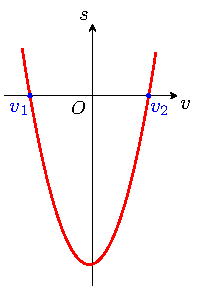
\includegraphics{Figures/budengshi2.pdf}
				\caption{}\label{fig:fig2}
			\end{center}
		\end{wrapfigure}
		根据题意，得
		\[
		\frac{1}{20}v + \frac{1}{180}v^2 > 39.5.
		\]
		移项整理，得
		\(
		v^2 + 9v - 7110 > 0.
		\)
		对于方程 \(v^2 + 9v - 7110 = 0\)，\(\Delta > 0\)，方程有两个实数根
		\[
		v_1 = \frac{-9 - \sqrt{28\,521}}{2}, \quad v_2 = \frac{-9 + \sqrt{28\,521}}{2}.
		\]
		画出二次函数 \(s = v^2 + 9v - 7110\) 的图象（图\ref{fig:fig2}），
		
		结合图象得不等式的解集为 \(\{v \mid v < v_1, \text{ 或 } v > v_2\}\)，从而原不等式的解集为
		\(
		\{v \mid v < v_1, \text{ 或 } v > v_2\}.
		\)
		
		因为车速 \(v > 0\)，所以 \(v > v_2\). 而 \(79.9 < v_2 < 80\)，所以这辆汽车刹车前的车速至少为 $80\; km/h$.
	\end{solve}
\end{frame}

\begin{frame}[t]{布置作业}
	
	P54--55 练习 ：1,2,3

	P55 习题2.3：4,6

\end{frame}

\end{document}
